\chapter{Observaties}

\section{Calibratie}
De resultaten van de calibratietest voor het aantal gebruikers kunnen gevonden worden in figuur \ref{fig:calibratie-gebruikers-resultaat}. Het aantal gebruikers wordt gekozen als het eerste moment waarop het de totale doorvoer vermindert, dit zorgt voor de gegevens in tabel \ref{table:calibratie-gebruikers-resultaat}. \todo{Check data in tabel}

\begin{table}[h!]
	\centering
	\begin{tabular}{l| l }
		\textbf{DBMS} & Aantal gebruikers \\
		\hline
		HBase & 40 \\
		MongoDB & 20\\
		Pgpool-II & 30\\
	\end{tabular}
	\caption{Calibratie: Aantal gebruikers per test voor de verschillende DBMS's}
	\label{table:calibratie-gebruikers-resultaat}
\end{table}

\begin{figure}[h!] 
\centering
	\subfigure[MongoDB]{\label{fig:calibratie-gebruikers-mongodb} \includegraphics[width=0.8\textwidth]{img/Observaties/threads-MongoDB}}
	\subfigure[Pgpool-II]{\label{fig:calibratie-gebruikers-pgpool-ii} 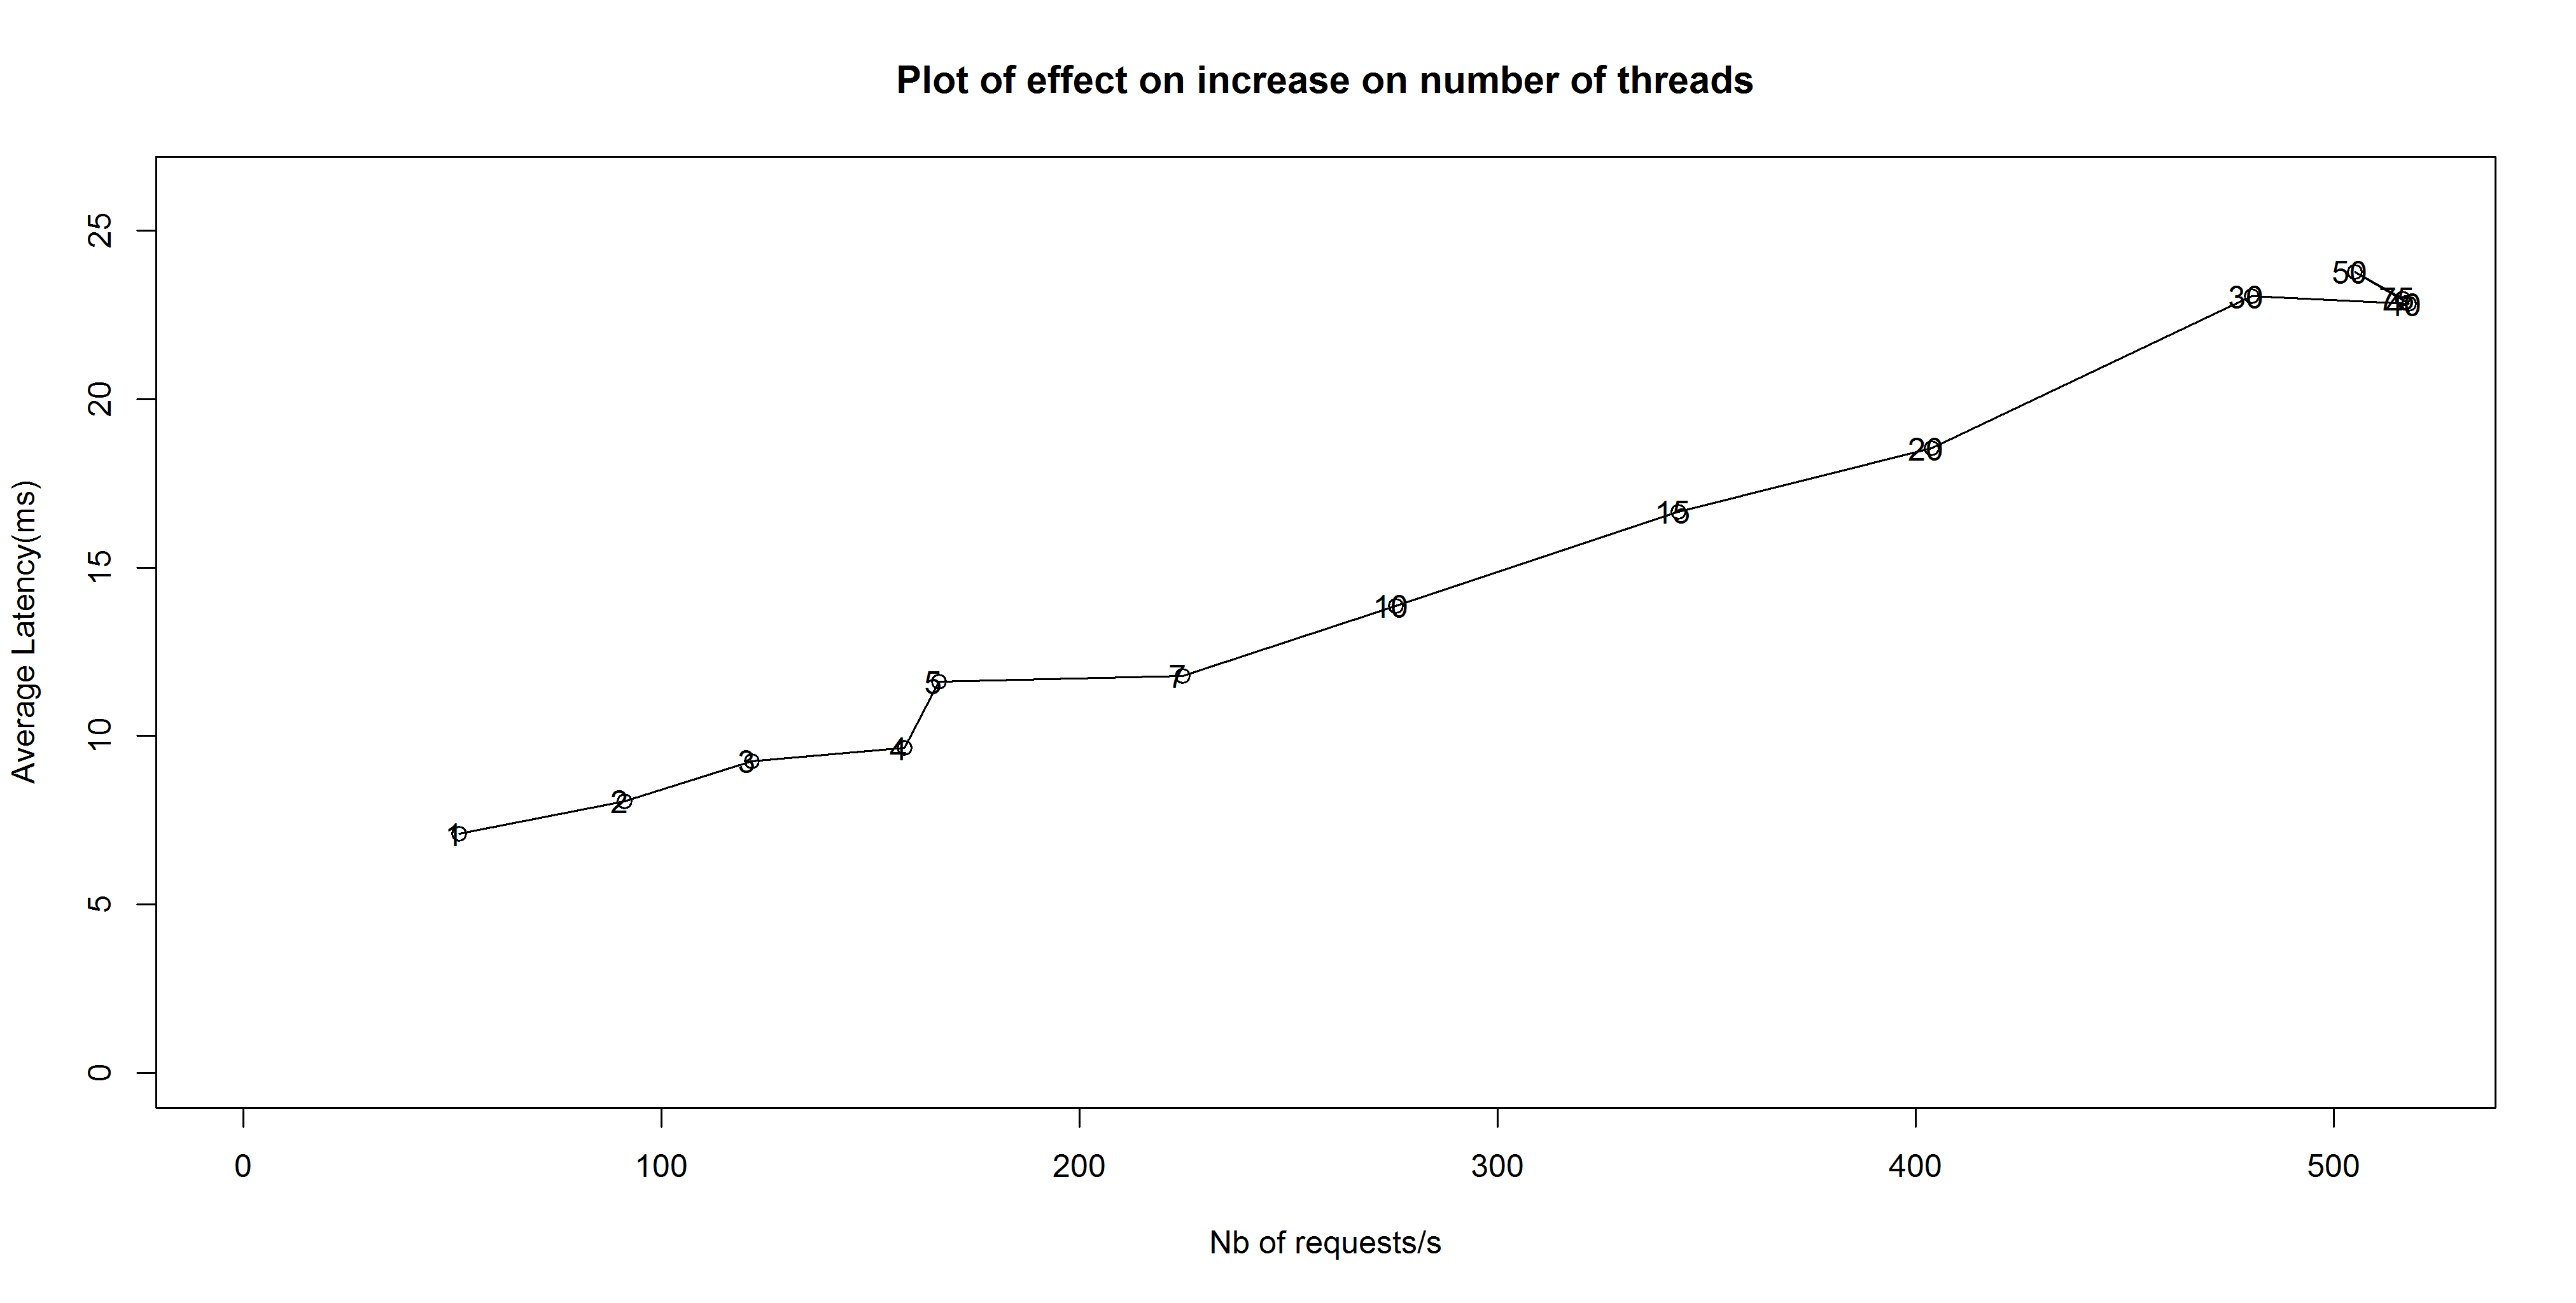
\includegraphics[width=0.80\textwidth]{img/Observaties/threads-postgresql}}
	\subfigure[HBase]{\label{fig:calibratie-gebruikers-hbase} \includegraphics[width=0.8\textwidth]{img/Observaties/threads-HBase}}
	\caption{Calibratie: Overzicht van het aantal requests tot de gemiddelde vertraging voor verschillend aantal gebruikers. Elk datapunt stelt een gebruiker voor met het aantal in het punt. }
	\label{fig:calibratie-gebruikers-resultaat}
\end{figure}

De resultaten voor de calibratietest voor het aantal requests per seconden kunnen gevonden worden in de figuren \ref{fig:calibratie-queriesperseconde-hbase}, \ref{fig:calibratie-queriesperseconde-mongodb} en \ref{fig:calibratie-queriesperseconde-pgpool-ii} voor respectievelijk HBase, MongoDB en Pgpool-II. Aan de hand van deze data wordt een getal gekozen voor het aantal queries per seconde zodat er een matige belasting is. Dit zorgt voor de gegevens in tabel \ref{table:calibratie-queriesperseconde-resultaat}.  \todo{Check data in tabel}

\begin{table}[h!]
	\centering
	\begin{tabular}{l| l }
		\textbf{DBMS} & Aantal requests per seconde \\
		\hline
		HBase & 200 \\
		MongoDB & 200\\
		Pgpool-II & 100\\
	\end{tabular}
	\caption{Calibratie: Aantal queries per seconde per test bij een matige belasting voor de verschillende DBMS's.}
	\label{table:calibratie-queriesperseconde-resultaat}
\end{table}

\begin{figure}[h!] 
	\centering
	\subfigure{\label{fig:calibratie-queriesperseconde-hbase-1} 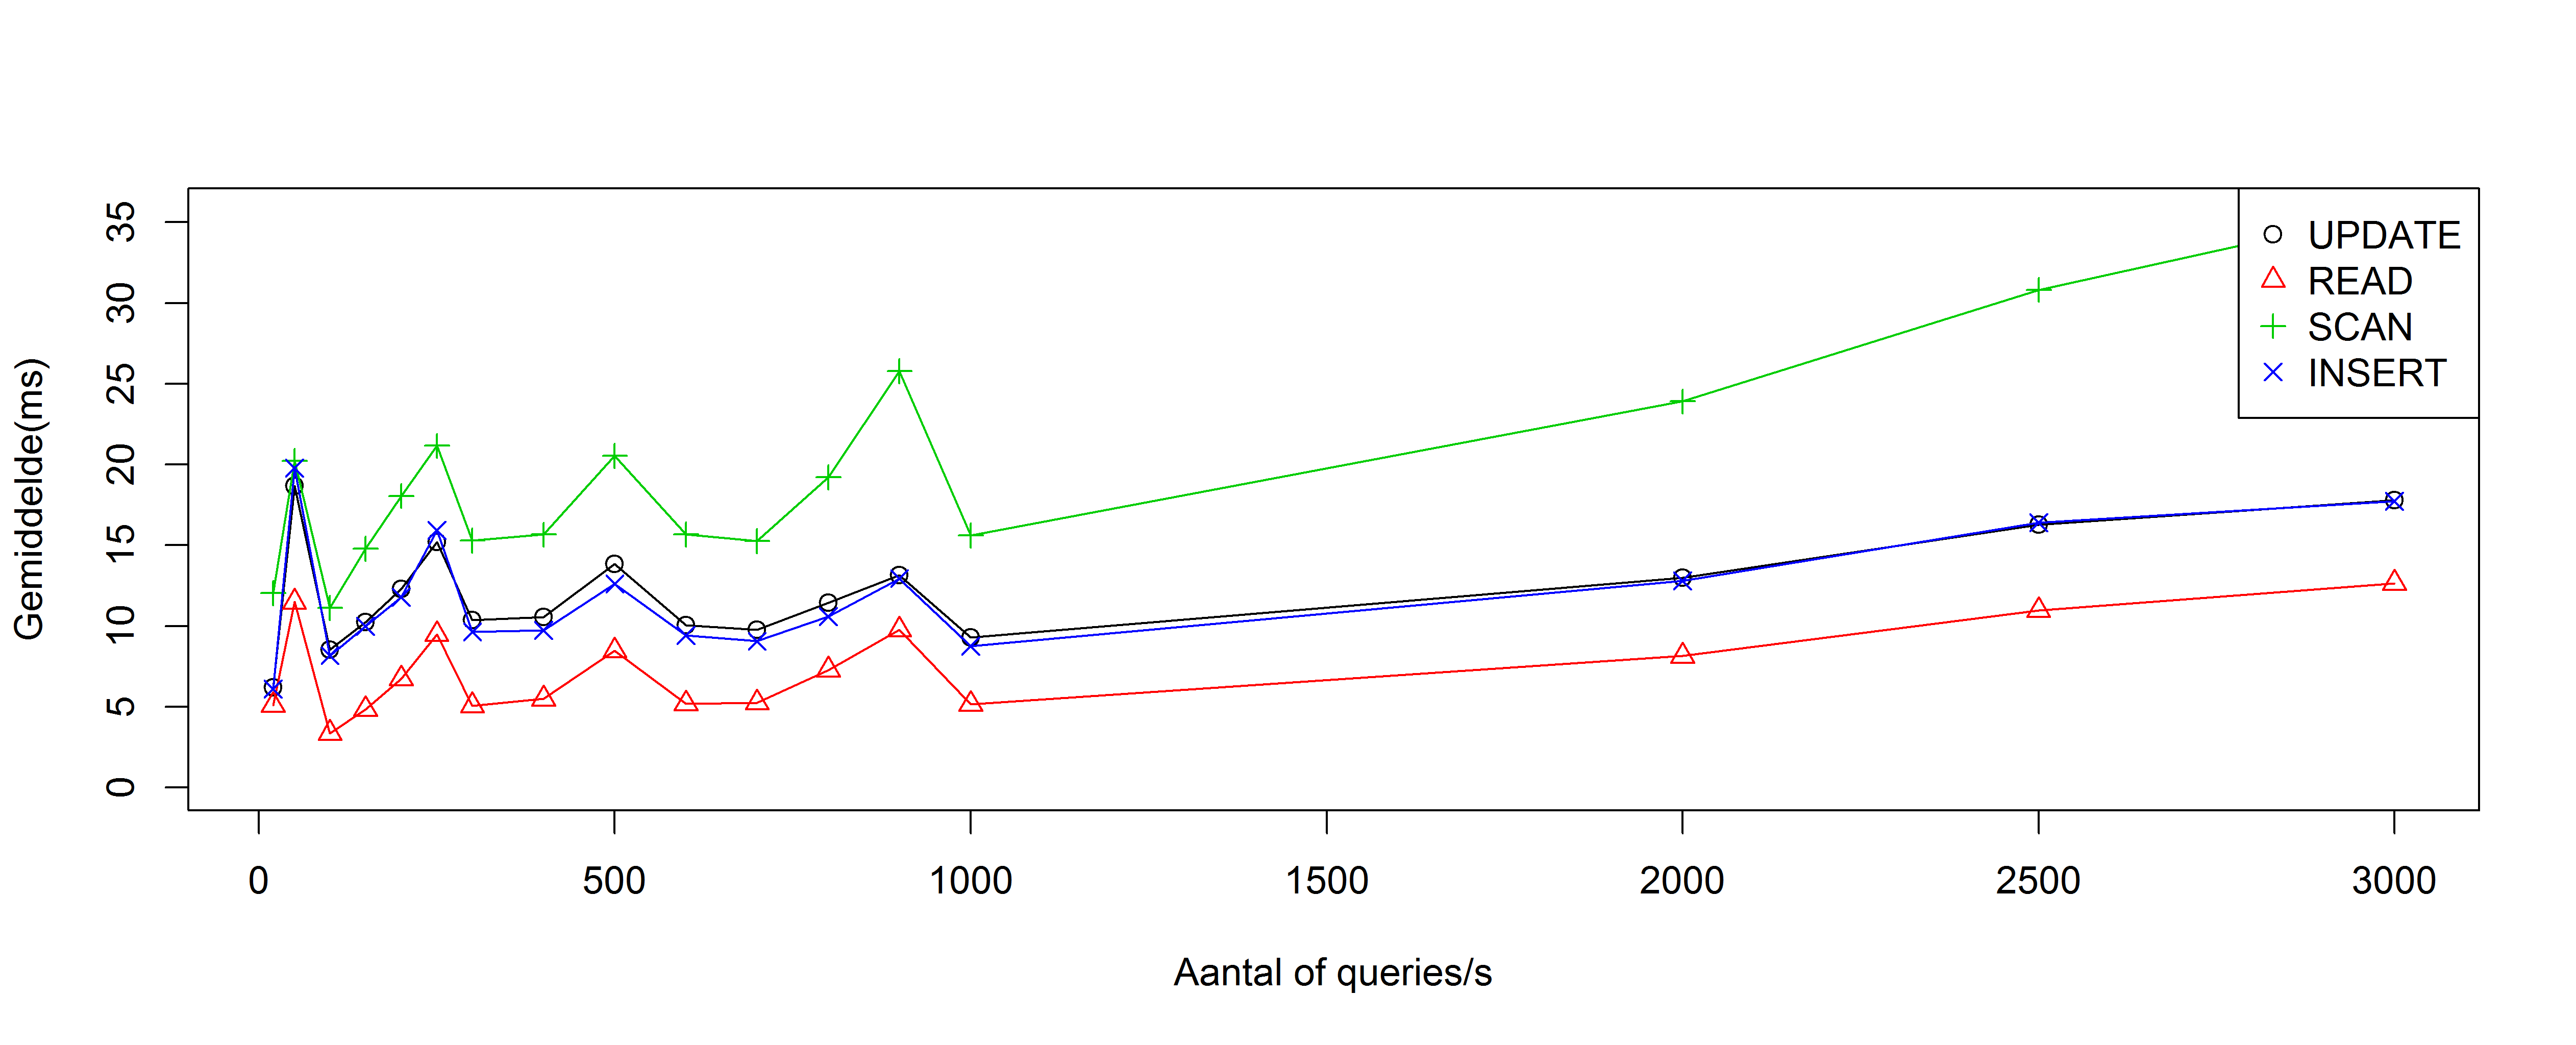
\includegraphics[width=0.8\textwidth]{img/Observaties/loadbalance-db-HBase}}
	\subfigure{\label{fig:calibratie-queriesperseconde-hbase-2} 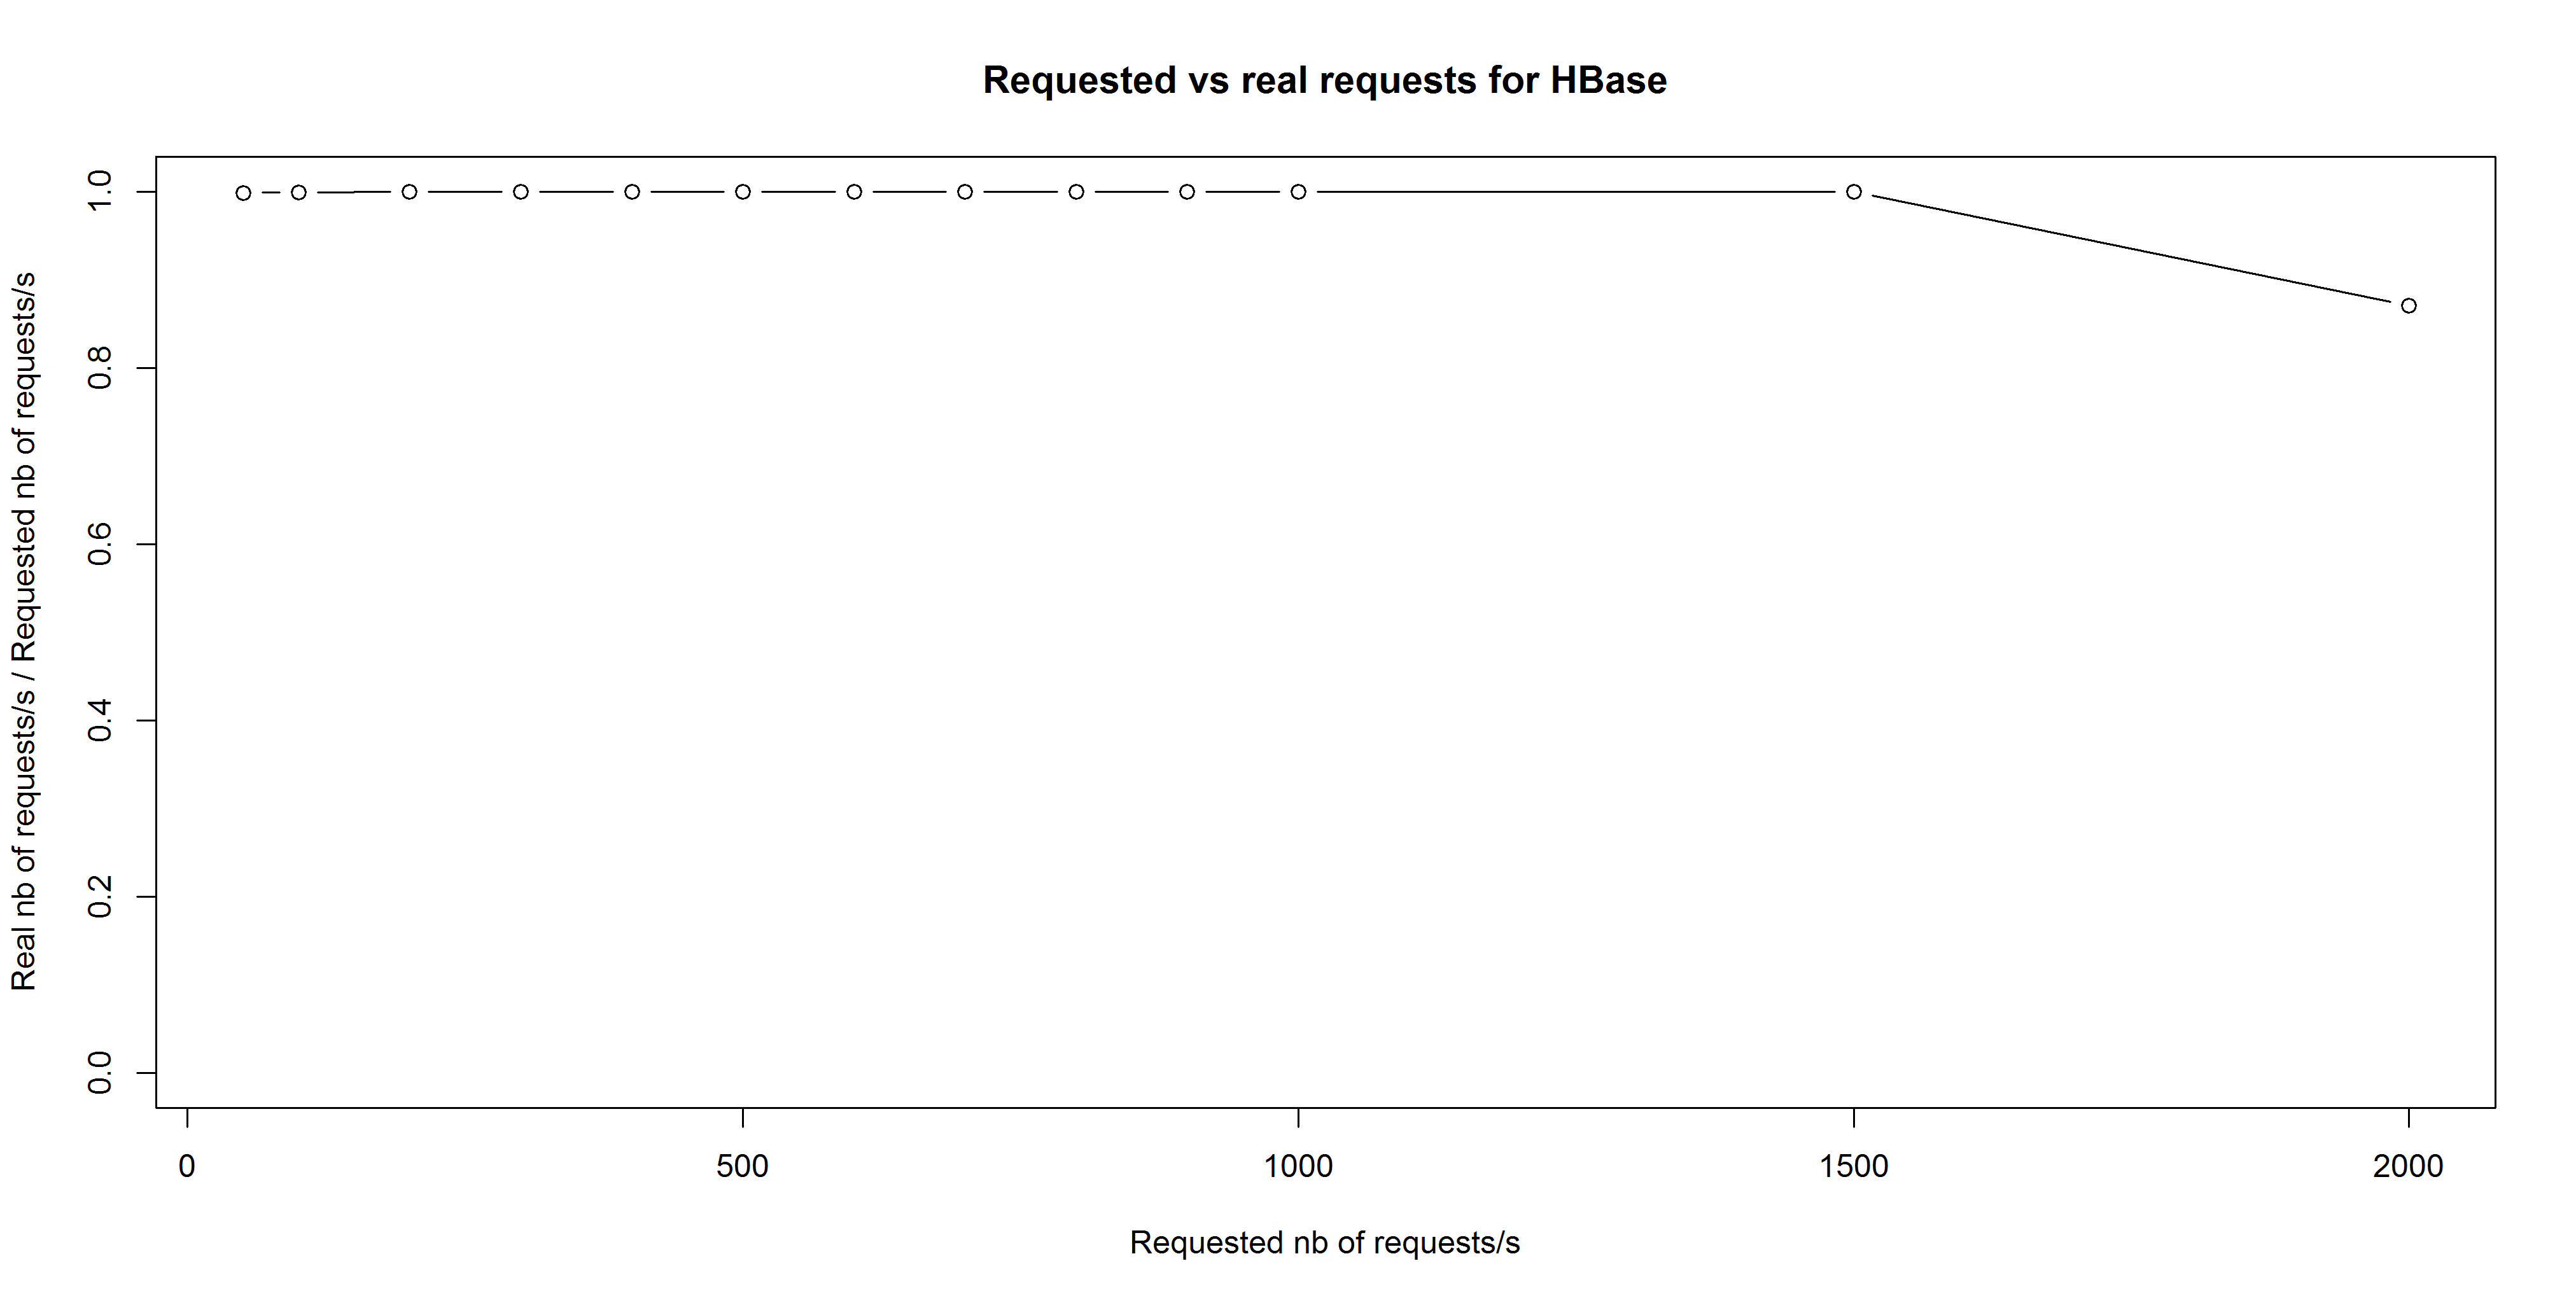
\includegraphics[width=0.8\textwidth]{img/Observaties/loadbalance-realthroughput-db-HBase}}
	\caption{Calibratie: Overzicht van de vertraging t.o.v. het theoretisch aantal aanvragen met een vergelijking hoeveel werkelijke aanvragen er waren voor HBase. }
	\label{fig:calibratie-queriesperseconde-hbase}
\end{figure}

\begin{figure}[h!] 
	\centering
	\subfigure{\label{fig:calibratie-queriesperseconde-mongodb-1} 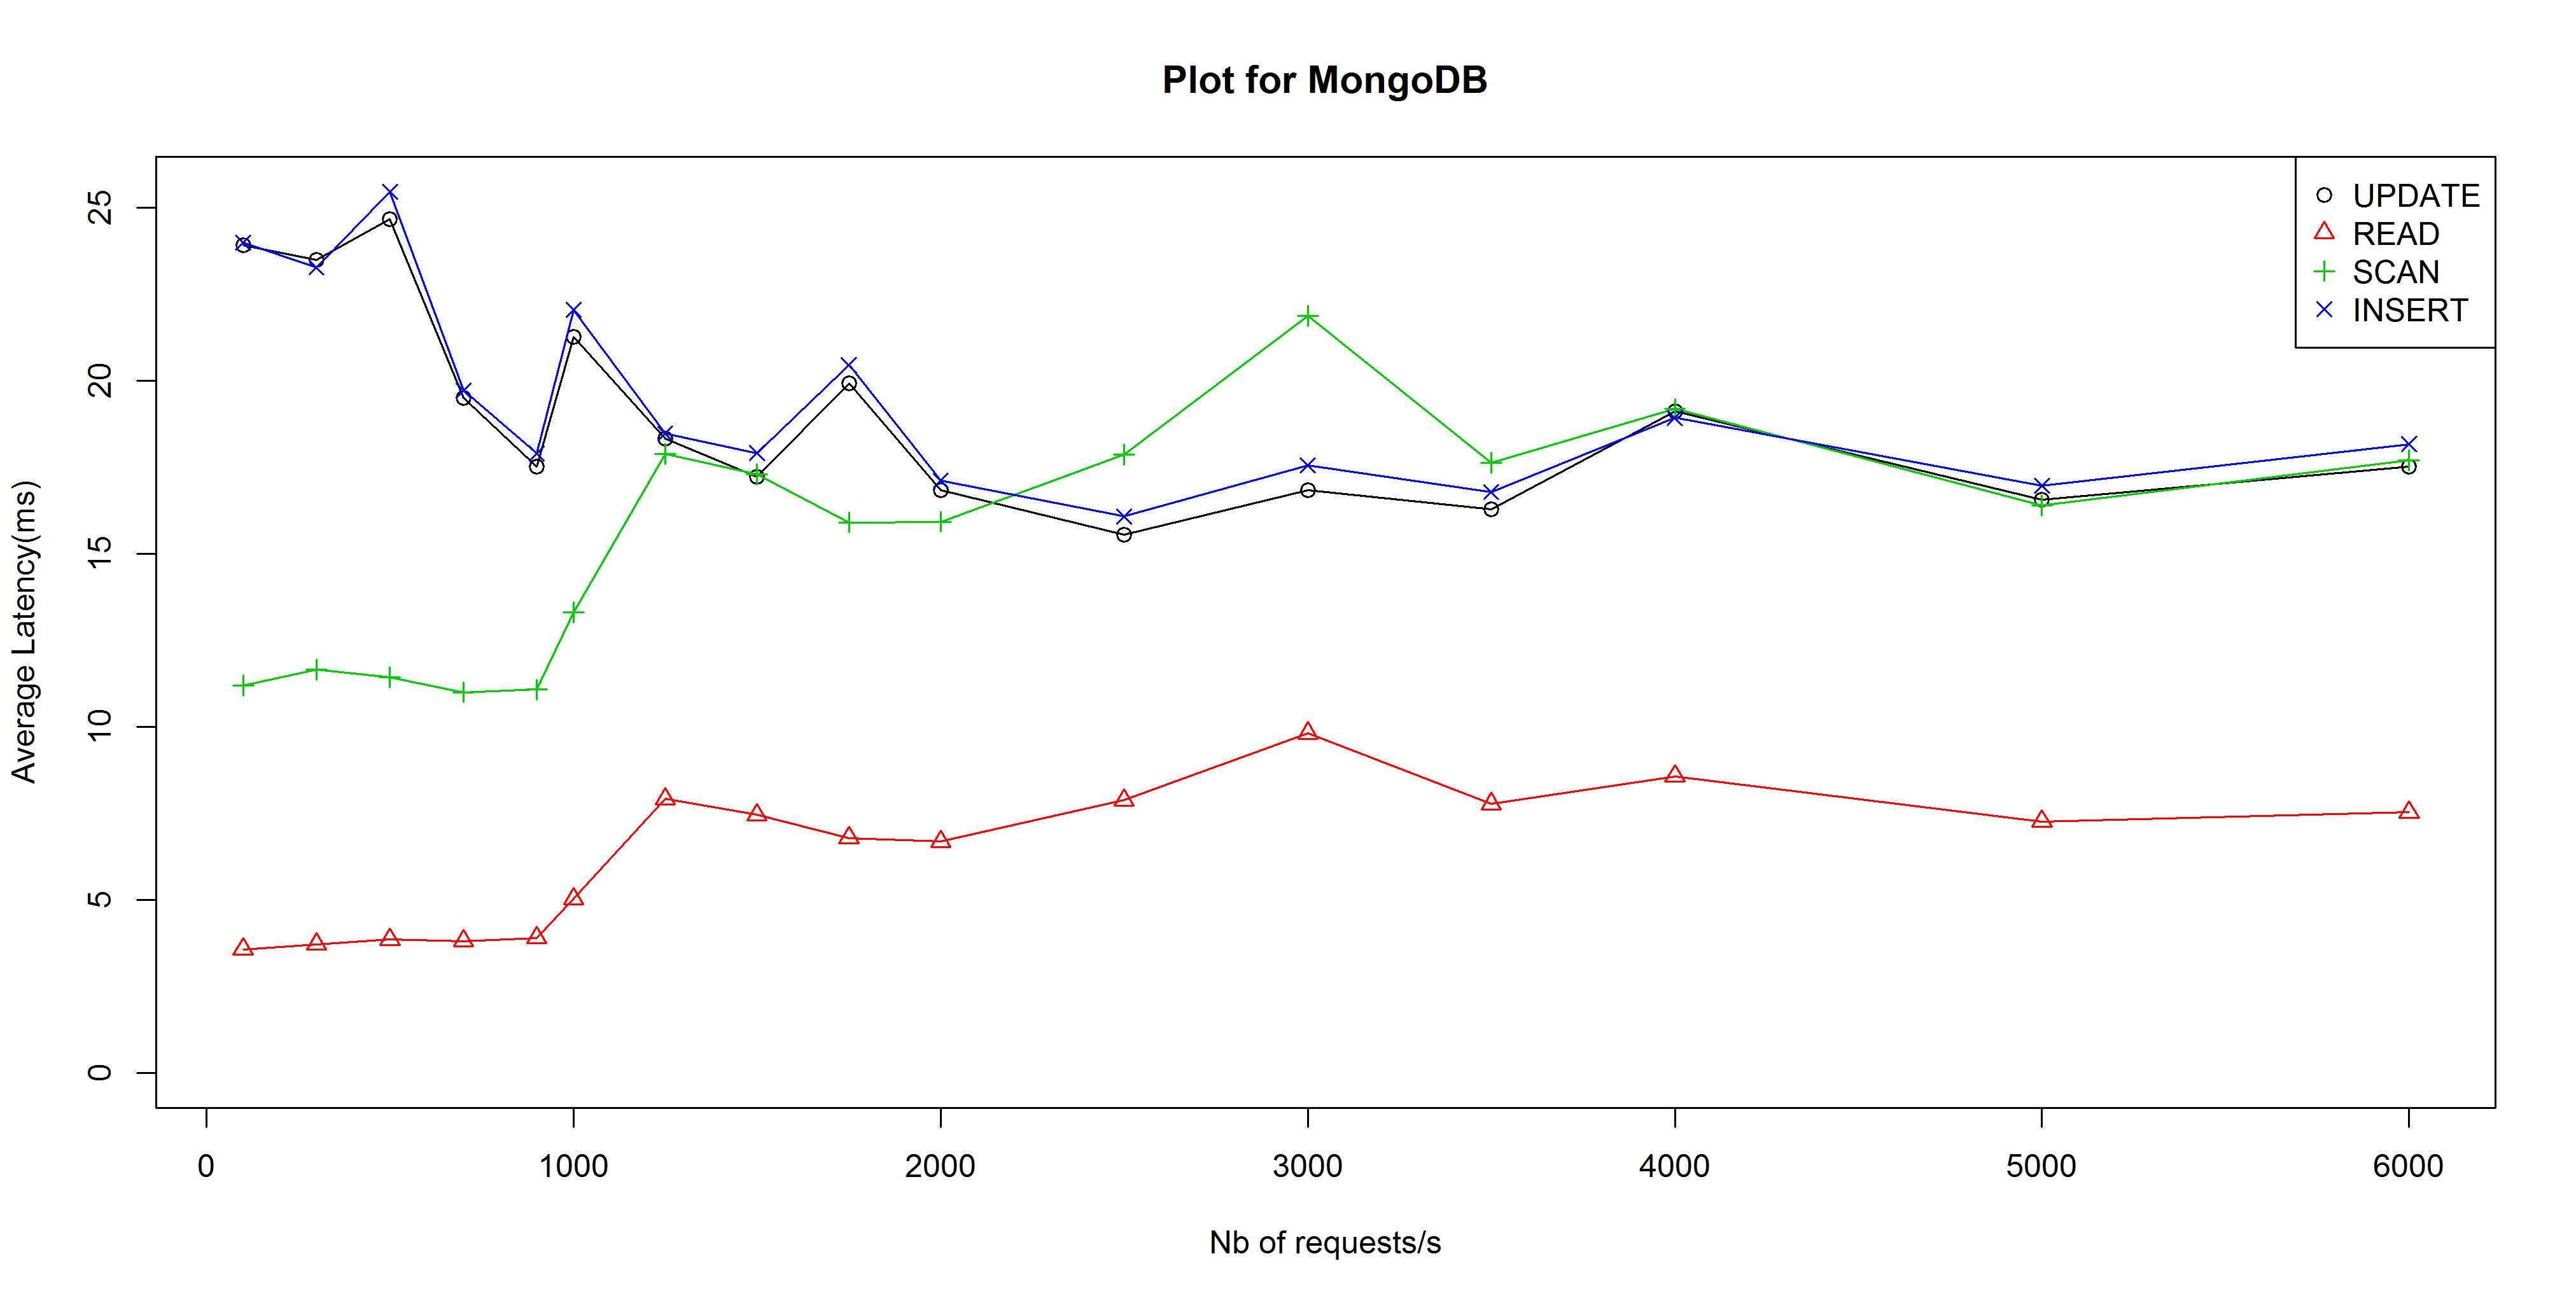
\includegraphics[width=0.8\textwidth]{img/Observaties/loadbalance-db-MongoDB}}
	\subfigure{\label{fig:calibratie-queriesperseconde-mongodb-2} 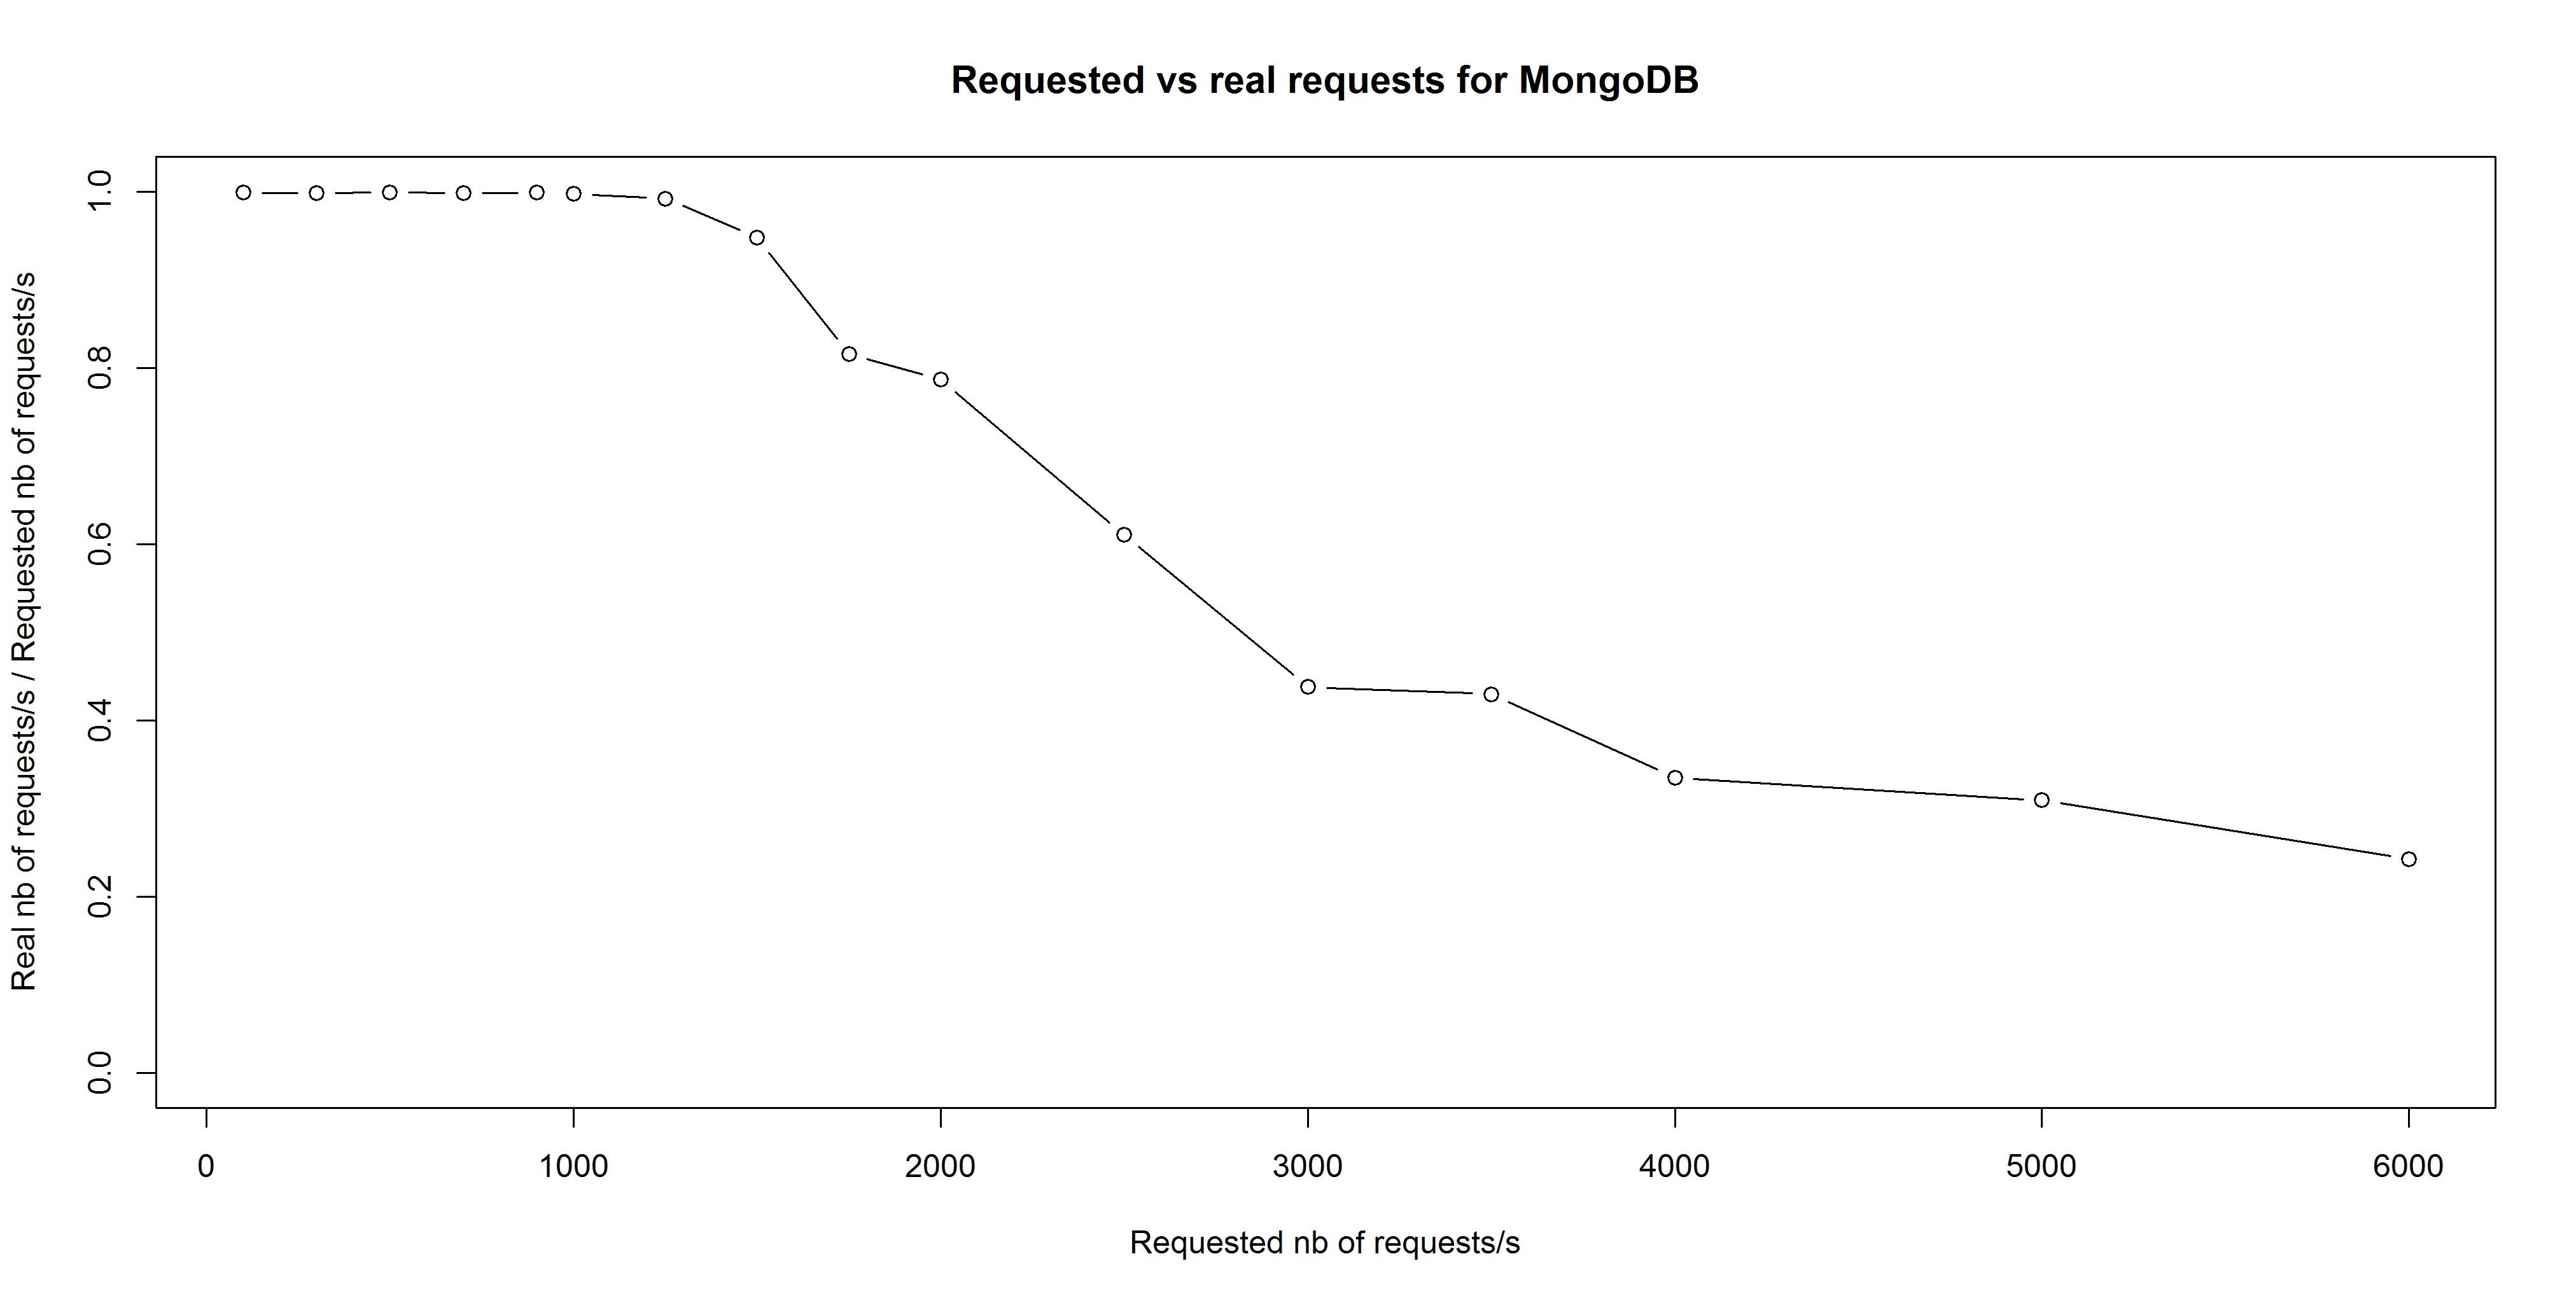
\includegraphics[width=0.8\textwidth]{img/Observaties/loadbalance-realthroughput-db-MongoDB}}
	\caption{Calibratie: Overzicht van de vertraging t.o.v. het theoretisch aantal aanvragen met een vergelijking hoeveel werkelijke aanvragen er waren voor MongoDB. }
	\label{fig:calibratie-queriesperseconde-mongodb}
\end{figure}

\begin{figure}[h!] 
	\centering
	\subfigure{\label{fig:calibratie-queriesperseconde-pgpool-ii-1} 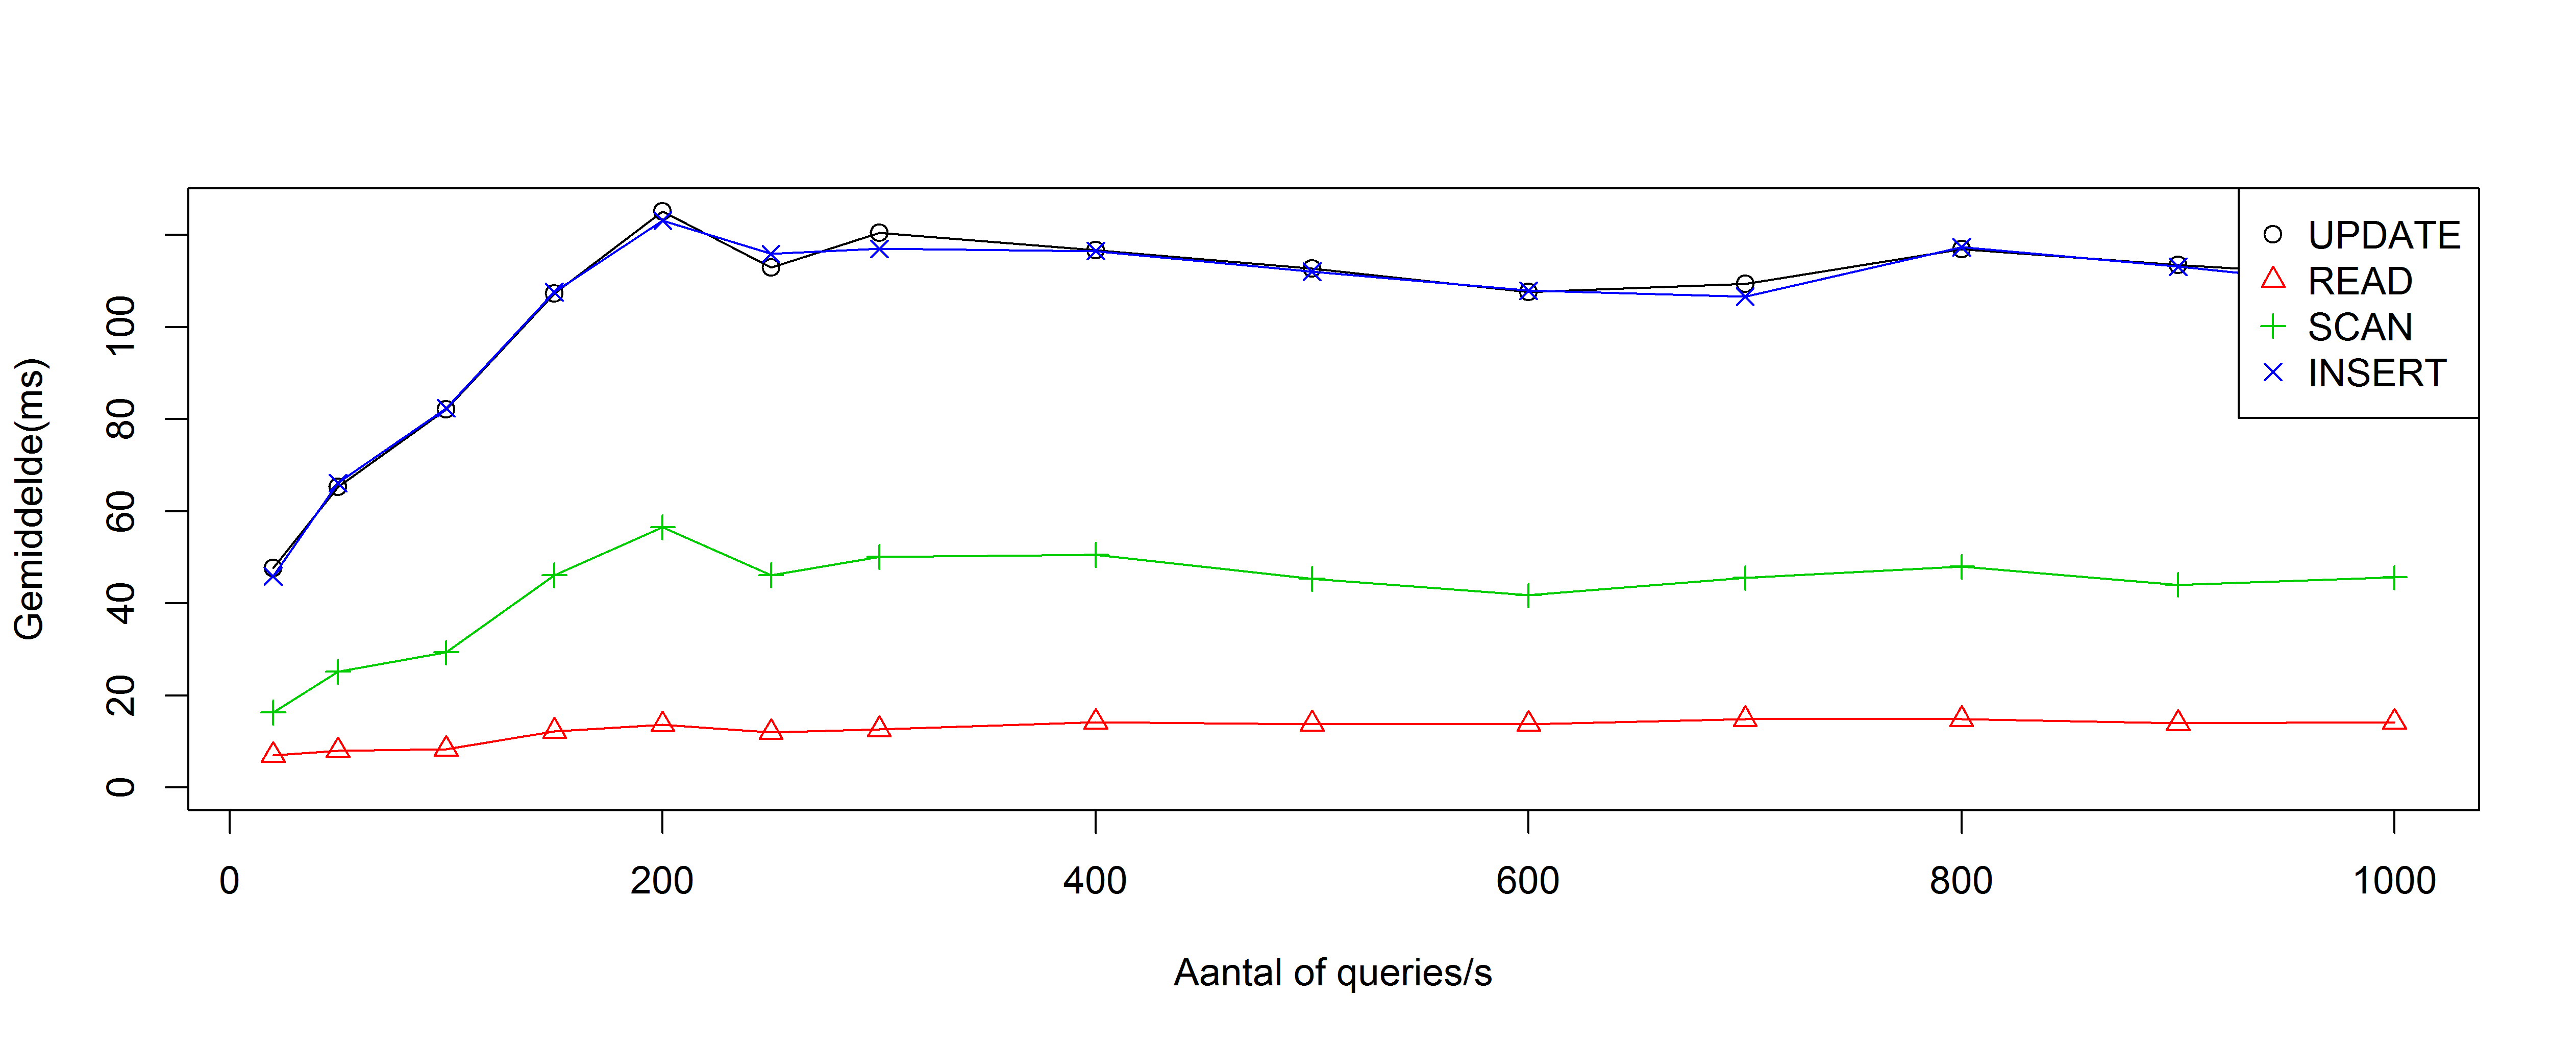
\includegraphics[width=0.8\textwidth]{img/Observaties/loadbalance-db-PostgreSQL}}
	\subfigure{\label{fig:calibratie-queriesperseconde-pgpool-ii-2} 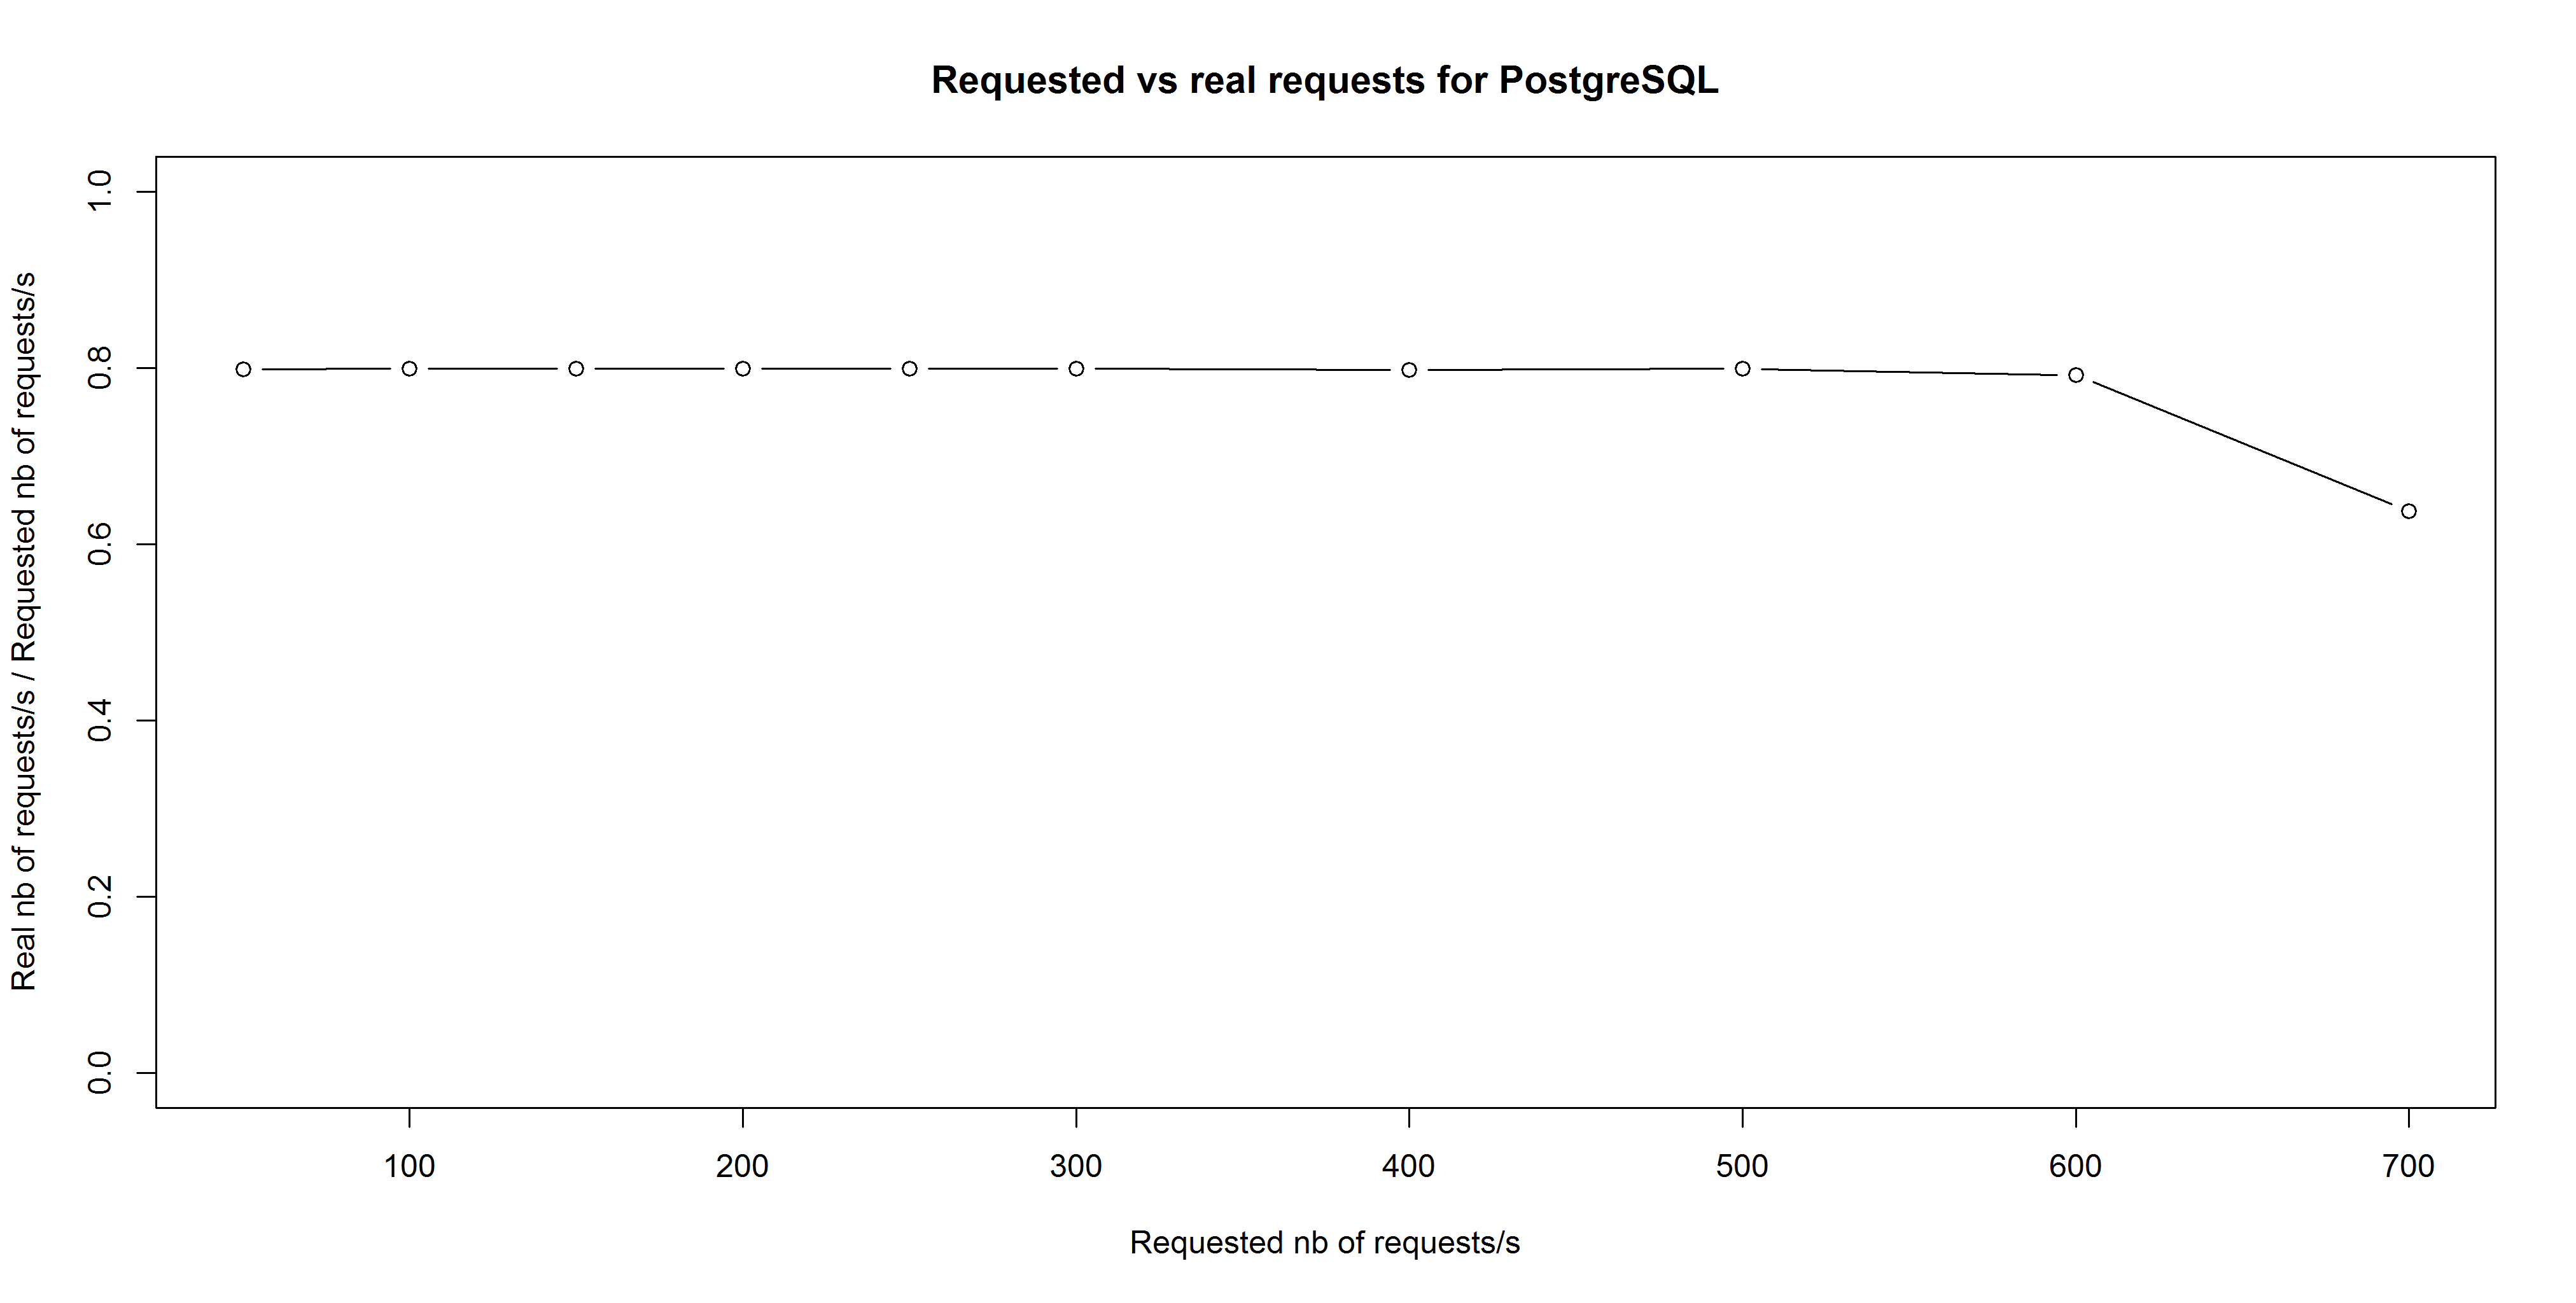
\includegraphics[width=0.8\textwidth]{img/Observaties/loadbalance-realthroughput-db-PostgreSQL}}
	\caption{Calibratie: Overzicht van de vertraging t.o.v. het theoretisch aantal aanvragen met een vergelijking hoeveel werkelijke aanvragen er waren voor Pgpool-II. }
	\label{fig:calibratie-queriesperseconde-pgpool-ii}
\end{figure}

\section{Beschikbaarheidstest}


\section{Consistentie test}
